\chapter{Esquema TT. Protección diferencial}
\section{Análisis del esquema TT}
En este esquema están conectados a tierra tanto el centro de la estrella del transformador como las masas. Se produce un defecto fase-tierra con tierra de retorno.
\begin{figure}[H]
	\centering
	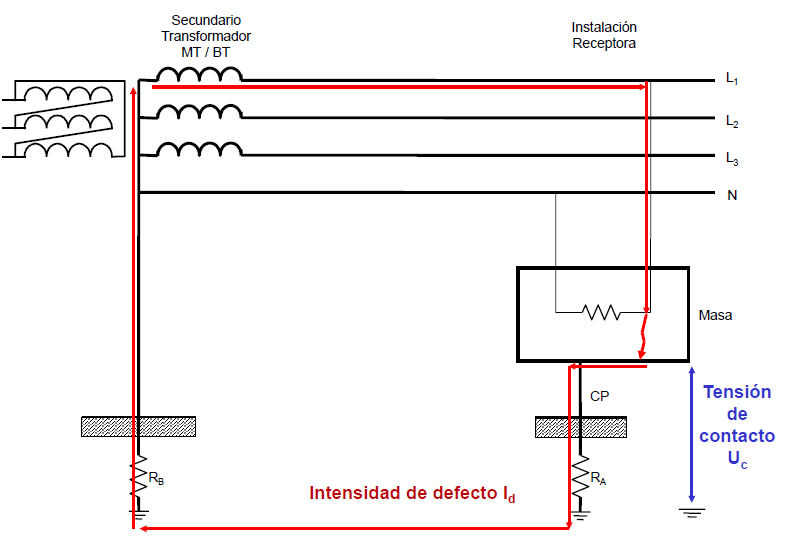
\includegraphics[width=0.5\linewidth]{Images/26}
	\label{fig:26}
\end{figure}

Su circuito equivalente es:
\begin{figure}[H]
	\centering
	\begin{adjustbox}{width=1\textwidth}
	
		\begin{circuitikz}
			\tikzstyle{every node}=[font=\normalsize]
			\draw (5.25,14.25) to[sinusoidal voltage source, sources/symbol/rotate=auto,l={ \normalsize $cU_{\text{fase-neutro}}$}] (5.25,11.25);
			\draw (6,15.5) to[european resistor,l={ \normalsize $\dfrac{2}{3} Z_{\text{media tension}}$}] (11,15.5);
			\draw (5.25,14.25) to[short] (5.25,15.5);
			\draw (5.25,15.5) to[short] (6.25,15.5);
			\draw (11,15.5) to[european resistor,l={ \normalsize $Z_{\text{trafo}}$}] (13.5,15.5);
			\draw (13.5,15.5) to[european resistor,l={ \normalsize $R_{\text{línea}}$}] (15.5,15.5);
			\draw (15.5,15.5) to[european resistor,l={ \normalsize $R_{\text{defecto}}$}] (15.5,12.75);
			\draw (15.5,12.75) to[european resistor,l={ \normalsize $R_{\text{cable protección}}$}] (15.5,10.75);
			\draw (15.5,10.75) to[european resistor,l={ \normalsize $R_{\text{puesta a tierra masas utilización}}$}] (15.5,8.5);
			\draw (5.25,11.25) to[european resistor,l={ \normalsize $R_{\text{puesta a tierra neutro}}$}] (5.25,8.5);
			\draw (5.25,8.5) to (5.25,8.25) node[ground]{};
			\draw (15.5,8.5) to (15.5,8.25) node[ground]{};
			\draw [ color={rgb,255:red,200; green,0; blue,255}, <->, >=Stealth] (14.25,13) -- (14.25,7.75)node[pos=0.5, fill=white]{$U_{contacto}$};
			\draw [ color={rgb,255:red,200; green,0; blue,255}, ->, >=Stealth] (8.5,14.75) -- (12.5,14.75)node[pos=0.5, fill=white]{$I_{defecto}$};
			\node [font=\normalsize, color={rgb,255:red,200; green,0; blue,255}] at (8.5,16.25) {$Z_{MT}$};
			\node [font=\normalsize, color={rgb,255:red,200; green,0; blue,255}] at (12.25,16.25) {$Z_T$};
			\node [font=\normalsize, color={rgb,255:red,200; green,0; blue,255}] at (14.5,16.25) {$R_F$};
			\node [font=\normalsize, color={rgb,255:red,200; green,0; blue,255}] at (16.5,14.5) {$R_d$};
			\node [font=\normalsize, color={rgb,255:red,200; green,0; blue,255}] at (16.5,12.25) {$R_{CP}$};
			\node [font=\normalsize, color={rgb,255:red,200; green,0; blue,255}] at (16.5,10) {$R_A$};
			\node [font=\normalsize, color={rgb,255:red,200; green,0; blue,255}] at (6.5,10.25) {$R_B$};
			\node [font=\normalsize, color={rgb,255:red,200; green,0; blue,255}] at (6.5,13.25) {$cU_0$};
		\end{circuitikz}
	\end{adjustbox}
	\label{fig:my_label}
\end{figure}

En estas condiciones:
\begin{equation}
	Z_{bucle}=\dfrac{2}{3}Z_{MT}+Z_T+Z_F+R_d+R_{CP}+R_A+R_B
\end{equation}
\begin{equation}
	I_d=\dfrac{c U_0}{Z_{bucle}}
\end{equation}
\begin{equation}
	U_c=\left(R_{CP}+R_A\right)I_d
\end{equation}
\subsection{Circuito equivalente simplificado en caso de fallo}
Normalmente las resistencias de puesta a tierra son mayores que el resto de impedancias:
\begin{equation}
	R_B+R'_A \ggg \dfrac{2}{3}Z_{MT}+Z_T+Z_F+R_d
\end{equation}

El caso más desfavorable desde el punto de vista de la protección:
\begin{equation}
	R_d=0
\end{equation}

La resistencia desde la masa de utilización a tierra:
\begin{equation}
	R_A'=R_A+R_{CP}
\end{equation}
\begin{center}
	\begin{figure}[H]
		\centering
	\begin{adjustbox}{width=0.5\textwidth}
		
		\begin{circuitikz}
			\tikzstyle{every node}=[font=\normalsize]
			\draw (5.25,14.25) to[sinusoidal voltage source, sources/symbol/rotate=auto,l={ \normalsize $cU_0$}] (5.25,11.25);
			\draw (5.25,14.25) to[short] (5.25,15.5);
			\draw (5.25,15.5) to[short] (6.25,15.5);
			\draw (15.5,10.75) to[european resistor] (15.5,8.5);
			\draw (5.25,11.25) to[european resistor] (5.25,8.5);
			\draw (5.25,8.5) to (5.25,8.25) node[ground]{};
			\draw (15.5,8.5) to (15.5,8.25) node[ground]{};
			\draw [ color={rgb,255:red,200; green,0; blue,255}, <->, >=Stealth] (14.25,10.75) -- (14.25,7.75)node[pos=0.5, fill=white]{$U_{contacto}$};
			\draw [ color={rgb,255:red,200; green,0; blue,255}, ->, >=Stealth] (8.5,14.75) -- (12.5,14.75)node[pos=0.5, fill=white]{$I_{defecto}$};
			\node [font=\normalsize, color={rgb,255:red,200; green,0; blue,255}] at (16.25,9.5) {$R_A$};
			\node [font=\normalsize, color={rgb,255:red,200; green,0; blue,255}] at (6,10) {$R_B$};
			\draw (6.25,15.5) to[short] (15.5,15.5);
			\draw (15.5,10.75) to[short] (15.5,15.5);
		\end{circuitikz}
	\end{adjustbox}
	\label{fig:my_label}
\end{figure}
\end{center}

En estas condiciones:
\begin{equation}
	R_S=R_{CP}+R_A+R_B
\end{equation}
\begin{equation}
	I_d=\dfrac{c U_0}{R_S}
\end{equation}
\begin{equation}
	U_c=\left(R_{CP}+R_A\right)I_d
\end{equation}

\textbf{Se debe disparar en caso de defecto mediante un interruptor diferencial.}
\section{Condiciones de protección}
\section{Interruptor diferencial}
\section{Selección de interruptores diferenciales}
\section{Selectividad entre interruptores diferenciales}
\section{Protección contra incendios}
\section{Ejemplo de cálculo de esquema TT}
\subsection{Datos de partida}
\subsection{Esquema eléctrico multifilar}
\subsection{Bucle de defecto}
\subsection{Circuito equivalente}
\subsection{Circuito equivalente simplificado}
\subsection{Cálculo de impedancia serie, corriente de defecto y tensión de contacto}
\subsection{Sensibilidad del interruptor diferencial}
\subsection{Comprobación del REBT esquema TT}
\subsection{Curvas de seguridad de tensión}
\subsection{Comprobar que se cumplen las curvas de seguridad de tiempo-intensidad}
